\chapter{Introduction}
\label{chap:introduction}

\chapterquote{There, sir! that is the perfection of vessels!}
{Jules Verne, 1828--1905}

%========================================================================================

The Standard Model has proven to be one of the greatest accomplishments of modern day particle physics.  It has have been used to make countless predictions of various physics processes across a wide range of energies that have proven to be consistent with experimental measurements.  The final piece of the Standard Model to be discovered was the Higgs boson, which was found by the ATLAS \cite{Aad:2012tfa} and CMS \cite{Chatrchyan:2012xdj} experiments at the Large Hadron Collider (LHC) in 2012.  

Despite the remarkable descriptive power of the Standard Model, there are a number of features in the universe that it does not provide a description for.  How does gravity fit into the Standard Model?  Why is there an excess of matter over antimatter in the observable universe?  How does the "dark matter" predicted by astronomers couple with the particles in the Standard Model?  What are the properties of the Higgs field in the Standard Model?  While the LHC and previous generations of particle collider experiment have had enormous success in validating the Standard Model and searching for new physics, it is clear that there is more work to be done. 

The linear collider experiments are proposals for the next generation of particle collider experiment.  They aim to provide precise measurements that will complement those made at the LHC and extend our understanding of particle physics.  One of the primary goals of the linear collider experiments is to study the Higgs field of the Standard Model.  A detailed description of the Higgs field is likely to help in the description of "dark matter" as many extensions of the Standard Model Higgs field contain particles that fit the properties of "dark matter".  The linear collider experiments will also provide a detailed description of the properties of the top quark.  This will complement the Higgs study as the strongest couplings for the Higgs in the Standard Model occurs with the top quark.  Another goal of the linear collider experiments is to provide high precision measurements of the electroweak sector in the Standard Model.  As the electroweak sector is the only place in the Standard Model where CP violation can occur, a detailed description will help to determine why there is an excess of matter over antimatter in the universe.  Furthermore, the linear collider will expand the descriptive reach for many Standard Model extensions such as supersymmetry (SUSY).

The linear collider experiments place emphasis on precision measurements.  As well as searching for beyond Standard Model physics, these precision measurements will guide the future direction of experimental particle physics.  Precision measurements have helped to guide the course of particle physics experiments in the past; LEP electroweak data, which gave indirect information about the lightness of the Higgs boson, was used to build the physics case for the LHC.  The precision measurements will be achieved through the application of particle flow calorimetry, which is a revolutionary technique in detector design that offers exceptional energy resolution for jets.  This paradigm shift means the linear collider detectors are significantly different from those found in previous generations of particle colliders.  As the detector design is continually evolving, the ongoing research in this area is vital for determining the overall success of these experiments.  

This thesis is organised as follows.  Chapter \ref{chap:anomalousgaugecouplingtheory} contains a summary of the Standard Model as well as an outline of the physics of interest related to the analysis presented in chapter \ref{chap:PhysicsAnalysis}.  Chapter \ref{chap:clicvertex} presents a study into a novel technology option for the Compact LInear Collider (CLIC) vertex detector.  Chapter \ref{chap:energyestimators} contains numerous studies related to the treatment of energy deposits in the linear collider simulation.  This begins with an outline of the calibration procedure for the linear collider detector simulation.  This is followed by a number of novel software techniques aimed at improving the energy resolution of a calorimeter designed for particle flow calorimetry.  Finally, the chapter concludes with a study of the timing requirements applied in the software trigger that will be used at the linear collider experiment.  Chapter \ref{chap:detopt} presents an optimisation study of the linear collider calorimeters.  The starkest contract in detector design when comparing particle flow calorimeter and tradition calorimeter is the design of the calorimeters.  As the linear collider experiments will be the first experiments purposefully built with particle flow calorimetry in mind, there is no precedence for the detector design.  Therefore, these studies are vital for guiding detector design.  Chapter \ref{chap:PhysicsAnalysis} contains a study into anomalous gauge couplings that are sensitive to massive gauge boson quartic vertices at the CLIC experiment.  This study is of particular interest as it provides a detailed probe of the electroweak symmetry breaking sector of the Standard Model as well as showing CLICs sensitivity to a possible extension to the Standard Model.  The thesis concludes with a summary in chapter \ref{chap:summary}.


%========================================================================================

%%%%%%% This is new!

\subsection{Experimental Conditions at CLIC}

The CLIC experiment will operate in a unique environment in comparison to previous generations of lepton colliders and this must be properly accounted for to get an accurate measure of the physics potential that CLIC has to offer.  The following aspects of the CLIC experiment present the largest challenges to the physics potential for the CLIC experiment:

\begin{itemize}
\item The high bunch charge density.  The small beam size at the impact point produces very large electromagnetic fields.  These fields can interact with the opposite beam particles causing them to radiate photons in an effect known as beamstrahlung.  Beamstrahlung acts to reduce the collision energy of the $\text{e}^{+}\text{e}^{-}$ pairs.   
\item Beam related backgrounds.  Beamstrahlung photons can subsequently interact to produce background events that must be accounted for.  Dominant backgrounds of this form that cannot be easily vetoed in the reconstruction include incoherent pair production of $\text{e}^{+}\text{e}^{-}$ and $\gamma\gamma \rightarrow \text{Hadron}$.  
\item Fast readout technology is crucial.  The CLIC bunch train consists of 312 bunches with a repetition rate of 50 Hz.  Each bunch is separated by 0.5ns, therefore, it will be necessary to integrate over multiple bunch crossing when reading out the detectors.  This places tight constraints on all detector electrical readout speeds and time resolutions.   
\end{itemize}

\subsubsection{Beam-Related Backgrounds at CLIC}
The primary sources of background for the CLIC experiment are as follows:
\begin{itemize}
\item $\text{e}^{+}\text{e}^{-}$ pair creation from the interaction of a beamstrahlung photons with the opposing beam.  The different mechanisms for pair creation are as follows:
\begin{itemize}
\item \textbf{Coherent pair production}.  This mechanism involves the interaction of a real beamstrahlung photon with the electromagnetic field from the opposing beam.
\item \textbf{Trident pair production}.  This mechanism involves the interaction of a virtual beamstrahlung photon with the electromagnetic field from the opposing beam.
\item \textbf{Incoherent pair production}.  This mechanism involves the interaction of a real or virtual beamstrahlung photon with the individual particles in the opposing beam.
\end{itemize}
\item $\gamma\gamma \rightarrow \text{Hadron}$ from the interaction of real or virtual beamstrahlung photons with each other.  Example Feynman diagrams for such processes is shown in figure ??. 
\item Beam halo muons that arise from interactions of the beam particles during collimation.  The dominant mechanisms producing beam halo muons are photon conversions into muon pairs ($\gamma \text{e}^{-} \rightarrow \mu^{+}\mu^{-}\text{e}^{-}$) and annihilation of positrons with atomic $\text{e}^{-}$ into muon pairs ($\text{e}^{+}\text{e}^{-} \rightarrow \mu^{+}\mu^{-}$) \cite{Pilicer:2015ijy}.
\end{itemize}

Each of these has to be properly addressed to get a true measure of the physics potential at CLIC.  Coherent and trident pair production is not a dominant source of background as they are produced at low transverse momenta, as figure \ref{fig:backgroundangle} shows, and a simple cut would veto these backgrounds.  This is not the case for incoherent pair production of $\text{e}^{+}\text{e}^{-}$, which are dominant in the forward regions of the detector, and $\gamma\gamma \rightarrow \text{Hadron}$, which are dominant in the tracker and the calorimeters (with the exception of low radii in the calorimeter endcaps) \cite{Linssen:2012hp, Sailer:2012mfa}.  Beam halo muons are not a major source of background either as they can be easily removed during the reconstruction due to the clear signal they create in the detector.  An algorithm was developed within the PandoraPFA framework for this purpose and it was found to be highly effective at removing the beam halo muons background \cite{Linssen:2012hp}.  

$\gamma\gamma \rightarrow \text{Hadron}$ events are the most dominant source of background to consider at CLIC as these events deposit more energy throughout the detector than incoherent pair production of $\text{e}^{+}\text{e}^{-}$ events \cite{Linssen:2012hp}.  The effect of the $\gamma\gamma \rightarrow \text{Hadron}$ background is incorporated into this analysis by overlaying $\gamma\gamma \rightarrow \text{Hadron}$ events onto the event samples used in this analysis.  The overlaid backgrounds are added prior to reconstruction so that their effect on the reconstruction is fully accounted for.  For a given event the exact number of background events overlaid is drawn from a Poisson distribution with a mean of 3.2 (1.3) events per bunch crossing at 3 (1.4) TeV.  While incoherent pairs are still a source of background they will produce a second order effect in comparison to the $\gamma\gamma \rightarrow \text{Hadron}$ events.

The PFO choices described in section \ref{sec:optimisationjetalgo} are applied to veto the effect of PFOs that arise from the overlaid $\gamma\gamma \rightarrow \text{Hadron}$ events.

\begin{figure}
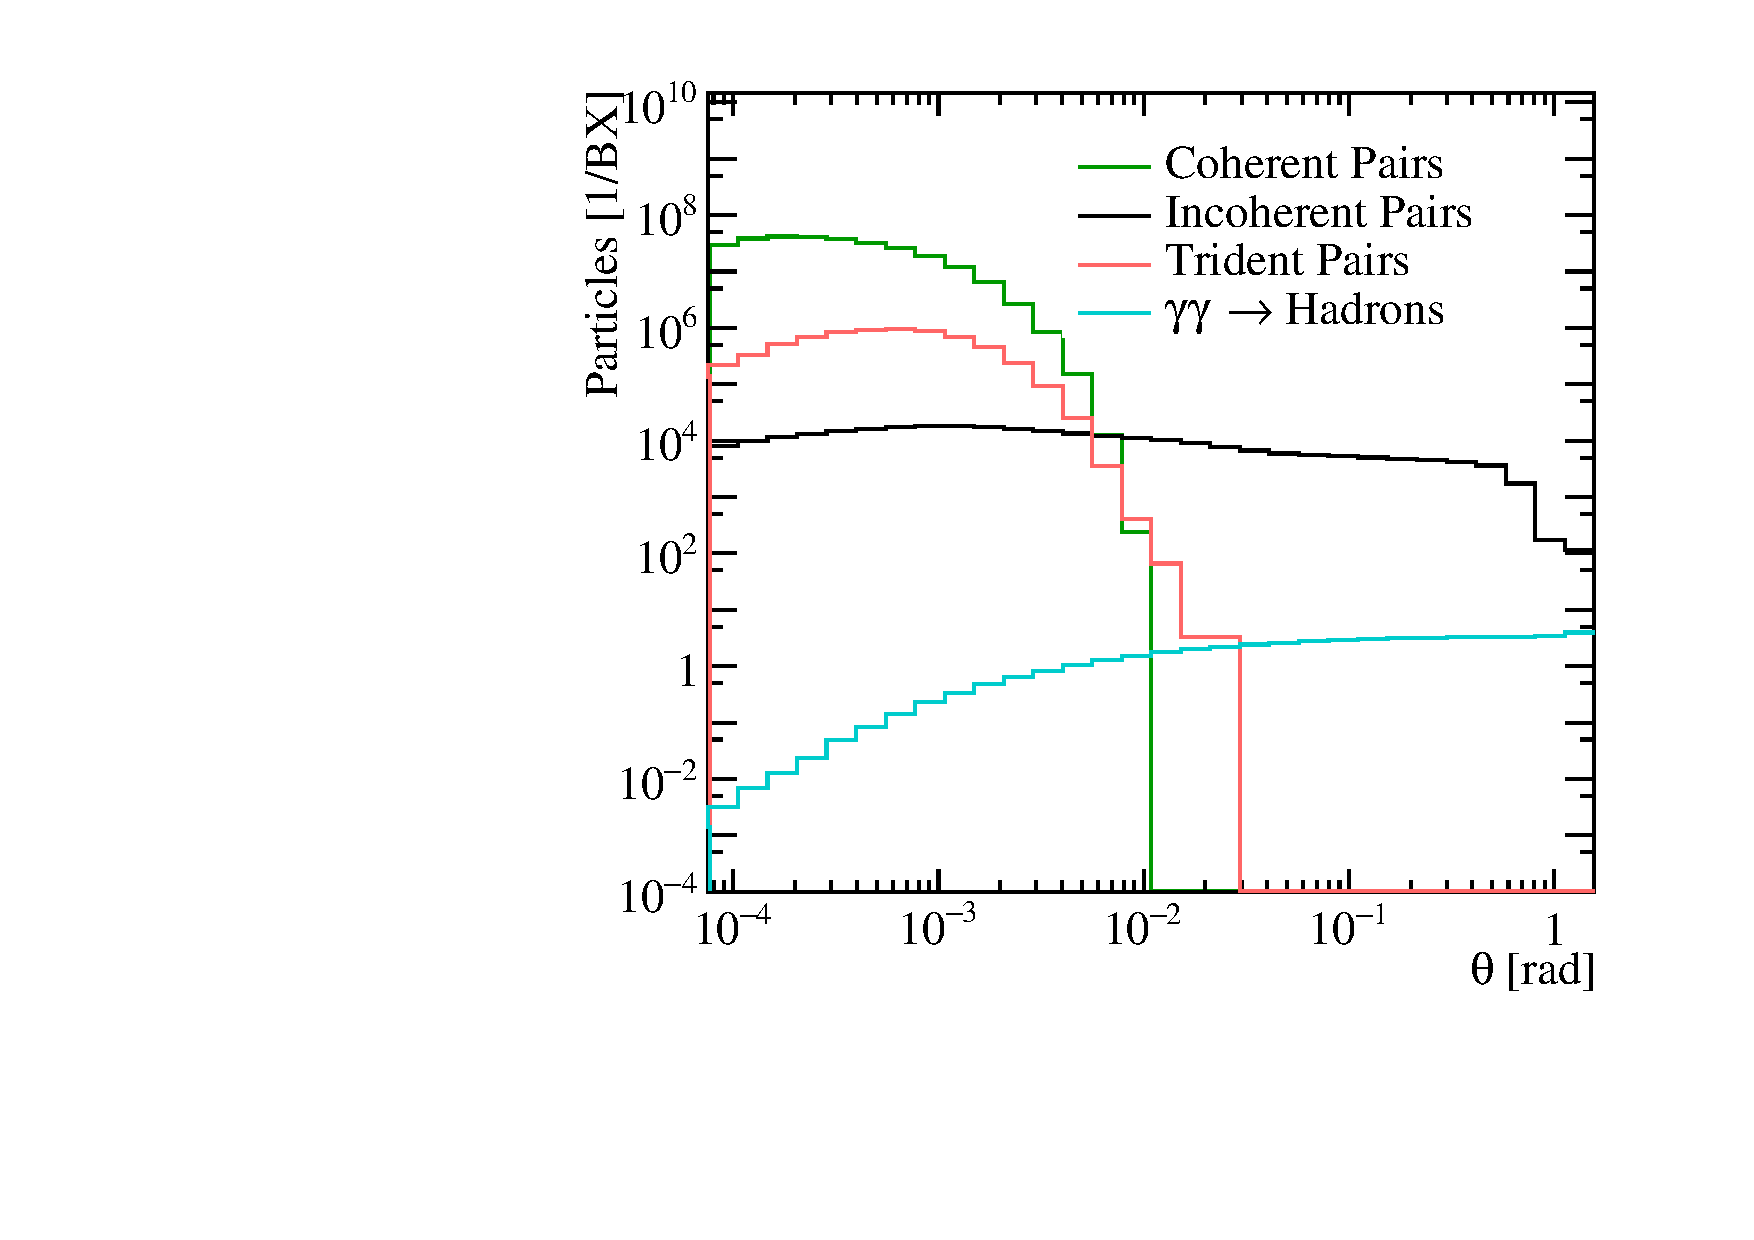
\includegraphics[width=0.5\textwidth]{FutureLinearColliders/Plots/CDRPlots/BackgroundAngleCut.pdf}
\caption[]{Angular distribution of number of particles for beam induced backgrounds for CLIC at $\sqrt{s} = 3$ TeV.  Taken from CLIC CDR.}
\label{fig:backgroundangle}
\end{figure}

%========================================================================================
%Physics introduction leading to chapter description.
%Max 2-3 pages
%Standard model extremely successful, missing gravity though
%Higgs discovery added crucial piece for mass generation
%Properties missing:
%Dark matter coupling
%CP violation -> Matter > antimatter
%ILC designed to study Higgs at 125 GeV, e+e-->Zh peak cross section at 250 GeV allows decay of Higgs to be measured by recoil of Z
%Top quark mass also studies.  Heaviest particle so coupling to H will be strong.
%Ultra-Precision for EW sector, which is only known CP violation 
%CLIC EW symmetry breaking at TeV scale
%and SUSY searches
%Improvement to LHC
%Precision Quantitative improvement of what is know , Jump in physics e.g. GUT in SUSY only proposed from precision EW  Lightness of Higgs from LEP electroweak data
%Discovery reach from processes with low production cross section at LHC
%Precision from PFlow
%Chapter Vertex
%Chapter Energy Est
%Chapter Calo Opt
%Chapter Physics Analysis
%========================================================================================